\documentclass[a4paper, 11pt]{article}
\usepackage[swedish]{babel}
\usepackage{hyperref}
\usepackage[margin=0.5in]{geometry}

\usepackage{graphicx}
\usepackage{amsmath}
\usepackage[arrowdel]{physics}
\usepackage{siunitx}

\newcommand{\integ}[5][]{\int\limits_{#2}^{#3}\dd[#1]{#4}#5}

\title{Sammanfattning av EL1000 Reglerteknik, allmän kurs}
\author{Yashar Honarmandi \\ yasharh@kth.se}
\date{\today}

\begin{document}

\maketitle

\begin{abstract}
	Detta ær en sammanfattning av kursen SH1014 Modern fysik.
\end{abstract}

\pagenumbering{roman}
\thispagestyle{empty}

\newpage

\tableofcontents

\newpage

\pagenumbering{arabic}

\section{Grundläggande koncept}

\paragraph{Syftet med reglerteknik}
Reglerteknik handlar om att kontrollera olika storheter, ofta betecknad $y$, i ett system mot något värde, ofta betecknad $r$. I tillägg till systemets egna beteende påverkas storheten vi vill reglera typiskt av en yttre störning $v$. Vi kan reglera systemet genom att tillföra en påverkan, ofta betecknad $u$.

\paragraph{Strategi}
För att förstå systemet, tar vi först fram en modell som beskriver det. Ur denna modellen fås typiskt en differentialekvation. Denna löser vi med Laplacetransform över tid.

\paragraph{Överförningsfungktionen}
För linjära system fås en lösning i Laplacerummet på formen $Y(s) = G(s)U(s)$, där $U$ är Laplacetransformen av $u$. Funktionen $G$ är överförningsfunktionen. Notera att denna lösningsformen typiskt beror på att alla initialvärden är $0$.

\paragraph{Poler}
Ett systems poler är rötterna till nämnarpolynomet (som typiskt finns) i överförningsfunktionen.

\paragraph{Stabilitet}
Ett system är stabilt om det tenderar mot ett visst läge efter lång tid. Systemets stabilitet är typiskt kopplad med dets poler. Detta kan man se i enkla fall, till exempel vanliga linjära ordinära differentialekvationer. Här är systemet stabilt om det inte finns några poler i högre halvplan, och avståndet längs med reella axeln anger hur snabbt lösningen tenderar mot det stabila läget.

\paragraph{Nollställen}
Ett systems nollställen är rötterna till täljarpolynomet (som typiskt finns) hos överförningsfunktioner. Eftersom vi är intresserade av att styra $y$, är det viktigt hur vi ska välja $u$ för att få det. Därmed är $\frac{1}{G}$ en viktig storhet, och nollställen kan därmed orsaka reglerproblem som är svårlösta.

\paragraph{Impulssvar}
Om lösningen för $Y$ är på formen $Y = GU$, är lösningen för $y$ på formen
\begin{align*}
	y(t) = \integ{0}{t}{\tau}{g(\tau)u(t - \tau)}.
\end{align*}
$g$ kallas för impulssvaret.

\paragraph{Blockschema}
Ett blockschema är ett systematisk sätt att rita reglerade system på. För att förstå hur man läser dem, betrakta figur \ref{fig:basic_block}.
\begin{figure}[!ht]
	\centering
	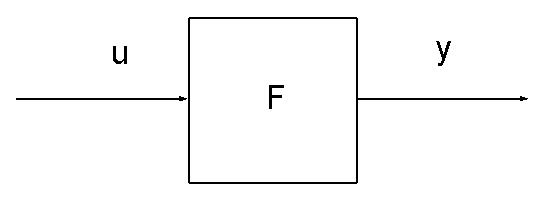
\includegraphics[width = 0.5\textwidth]{./Images/basic_block.eps}
	\caption{Illustration av ett enkelt blockschema.}
	\label{fig:basic_block}
\end{figure}

Med denna figuren menas att $Y(s) = F(s)U(s)$.

\paragraph{Rotort}
En rotort är en plott av ett systems poler som funktion av någon parameter. Den är typiskt uppdelad i grenar, som är kurvor i planet som är parametriserade av parametervärdet. Polerna som motsvarar parametervärdet $0$ är rotortens startpunkter, och polarna motsvarande parametervärdet $\infty$ är rotortens ändpunkter. Om rotorten närmar sig kurvor, är dessa rotortens asymptoter.

\section{Prestanda och prestandamått}

\paragraph{Stigtid}
Stigtiden definieras som $T_{\text{r}}, = t_{2} - t_{1}$, där vi typiskt har kriteriet $y(t_{2}) = 0.9$ och $y(t_{1}) = 0.1$, med $y$ mätt i relativa enheter.

\paragraph{Insvängningstid}
Insvängningstiden definieras som $\abs{y(t) - 1} < p$ när $t > T_{\text{s}}$, med $y$ mätt i relativa enheter. $p$ är typiskt lika med $0.05$.

\paragraph{Översläng}
Överslänget definieras som $y_{\text{max}} - 1$, med $y$ mätt i relativa enheter.

\paragraph{Parametrar i svängningslika system}
Om du har ett system med ett andra ordningens polynom i överförningsfunktionens nämnare, skriv polynomet som $s^{2} + 2\zeta\omega_{0}s + \omega_{0}^{2}$. $\omega_{0}$ är systemets resonansfrekvens och $\zeta$ dets dämpning. Det gäller för ett rent andra ordningens system att
\begin{align*}
	T_{\text{r}} \propto \frac{1}{\omega_{0}},\ T_{\text{s}} \approx \frac{3}{\zeta\omega_{0}},\ M = e^{\frac{\pi\zeta}{\sqrt{1 - \zeta^{2}}}}.
\end{align*}

\paragraph{Stationärt fel}
Det stationära felet är felet $e = r - y$ som kvarstår efter lång tid.

\paragraph{Felkoefficienter}
Det stationära felet beror både på systemets egenskaper och reglersignalen. Om reglersignalen är på formen $r_{n} = t^{n}\theta(t)$, där $\theta$ är Heavisidefunktionen, definieras felkoefficienterna som
\begin{align*}
	e_{n} = \lim\limits_{t\to\infty}r_{n} - y.
\end{align*}

\section{Blockschema}

\paragraph{Syftet med blockschema}
Blockschema är ett systematisk sätt att rita reglerade system på.

\paragraph{Hur funkar det?}
Betrakta blocket i figur \ref{fig:basic_block}.

\begin{figure}[!ht]
	\centering
	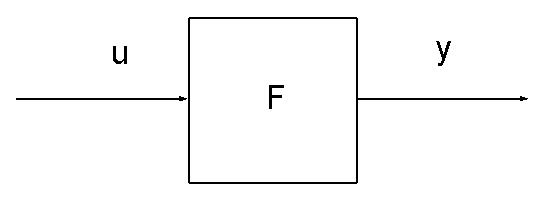
\includegraphics[width = 0.5\textwidth]{./Images/basic_block.eps}
	\caption{Illustration av ett enkelt block i ett blockschema.}
	\label{fig:basic_block}
\end{figure}

Med denna figuren menar vi exakt att $Y(s) = F(s)U(s)$.

\section{Negativ återkoppling}

\paragraph{Vad är negativ återkoppling?}
I denna kursen kommer vi att studera hur man kontrollerar ett system vid att låta avvikelsen mot det önskade värdet kontrollera regleringen av storheten.

\paragraph{Illustration i blockdiagram}
Ett enkelt negativt kontrollsystem illustrearas i figur \ref{fig:negative_feedback}.

\begin{figure}[!ht]
	\centering
	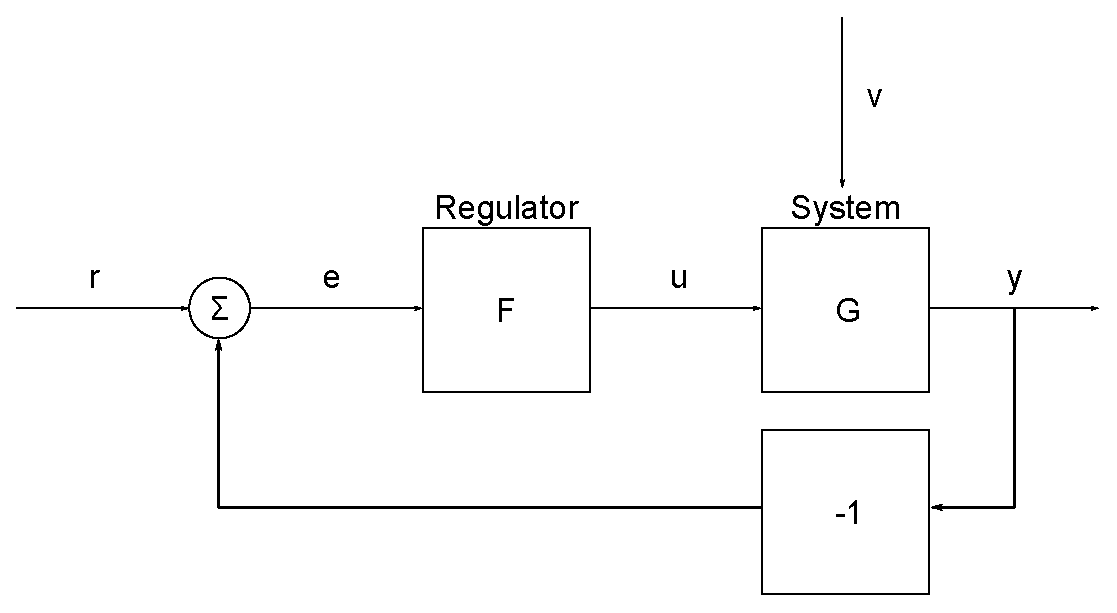
\includegraphics[width = \textwidth]{./Images/negative_feedback.eps}
	\caption{Schematisk illustration av ett enkelt negativt återkopplad system.}
	\label{fig:negative_feedback}
\end{figure}

\paragraph{Beskrivning av systemet}
Vi börjar beskrivningen av systemet med att inte betrakta störningar. I ena ändpunkten har vi
\begin{align*}
	Y = GU = GFE.
\end{align*}
Summationskomponenten till vänster ger oss
\begin{align*}
	E = R - Y,
\end{align*}
och därmed
\begin{align*}
	Y = GFR - GFY.
\end{align*}
Därmed kan vi skriva
\begin{align*}
	Y = \frac{GF}{1 + GF}R.
\end{align*}

\paragraph{Återkopplad överföringsfunktion}
För ett återkopplad system som kan skrivas som $Y = G_{\text{C}}R$ definieras $G_{\text{C}}$ som den återkopplade överföringsfunktionen. För systemet ovan har vi alltså
\begin{align*}
	G_{\text{C}} = \frac{GF}{1 + GF}R.
\end{align*}

\paragraph{Samband mellan reglerfel och referens}
Alternativt kan vi lösa systemet ovan för att få
\begin{align*}
	R - E = GFE,\ E = \frac{1}{1 + GF}R.
\end{align*}

\paragraph{Samband mellan referens och insignal}
Systemet ovan kan även lösas för att ge
\begin{align*}
	U = FR - FY = FR - GFU,\ U = \frac{F}{1  + GF}R.
\end{align*}

\paragraph{Slutna systems poler}
Vi ser att slutna system har poler där $1 + GF = 0$. Därmed bestäms systemets stabilitet av systemet och regulatorn.

\section{Frekvensanalys}

\paragraph{Fundamental ide}
Eftersom periodiska funktioner kan skrivas som en summa av trigonometriska funktioner och funktioner som avtar tillräcklig snabbt kan skrivas som en integral över trigonometriska funktioner, vet vi att när vi studerar linjära system räcker det att studera systemets respons på en enda term, alltså en enda trigonometrisk funktion, och se hur den beror av frekvensen. Om vi tillför en signal $u = \sin{\omega t}$ till ett system med överförningsfunktion $G$ får vi
\begin{align*}
	y &= \integ{0}{\infty}{\tau}{g(\tau)u(t - \tau)} \\
	  &= \Im\left(\integ{0}{\infty}{\tau}{g(\tau)e^{i\omega(t - \tau)}}\right) \\
	  &= \Im\left(e^{i\omega t}\integ{0}{\infty}{\tau}{g(\tau)e^{-i\omega\tau}}\right) \\
	  &= \Im(e^{i\omega t}G(i\omega)) \\
	  &= \abs{G(i\omega)}\sin(\omega t + \arg{G(i\omega)}).
\end{align*}
Det kan även finnas transienta termer här, men om systemet är stabilt kommer dessa försvinna över tid. Vi ser alltså att systemets svar beror av $G(i\omega)$.

\paragraph{Nyquistdiagram}
Ett Nyquistdiagram är en uppritning av $G(i\omega)$ för $0 < \omega < \infty$.

\paragraph{Bodediagram}
Ett Bodediagram är en uppritning av $\abs{G(i\omega)}$ och $\arg{G(i\omega)}$ som funktioner av $\omega$.

\paragraph{Bandbredd}
Bandbredden är bredden på det frekvensintervallet där $\abs{G(i\omega} \geq \frac{1}{\sqrt{2}}$, och benämnas $\omega_{\text{B}}$. Bandbredden kan ge information om systemets tillväxt, då hög bandbredd typiskt betyder snabb tillväxt. Man önskar typiskt att denna skall vara stor.

\paragraph{Resonansfrekvens}
Resonansfrekvensen $\omega_{\text{r}}$ är den frekvens som ger starkast respons i systemet.

\paragraph{Resonanstopp}
Resonanstoppen är $M_{\text{p}} = \abs{G(i\omega_{\text{r}})}$, och ger typiskt en indikation på hur mycket översläng man får. Man önskar typiskt att denna ska vara liten.

\paragraph{Stationärt fel}
Det stationära felet ges av $e_{0} = 1 - G_{\text{C}}(0)$.

\paragraph{Brytningspunkter}
Om överförningsfunktionen kan skrivas som
\begin{align*}
	G(i\omega) = \frac{\prod(i\omega - z_{i})}{\prod(i\omega - p_{i})},
\end{align*}
är alla $z_{i}$ och $p_{i}$ brytningspunkter för systemet. Här kommer de största lutningsändringarna i Bodediagrammet.

\paragraph{Bodes relation}
Låt $G$ vara minimumsfas, dvs. ha alla sina nollställen och poler i vänstre halvplan, och $G(0) > 0$. Då gäller att om $\abs{G(i\omega)}$ i ett visst frekvensområde avtar med \SI{20}{\deci\bel} per dekad (en dekad är en ökning i frekvens med en faktor $10$), är $\arg{G(i\omega)}\approx \SI{-90}{\degree}$, och om $\abs{G(i\omega)}$ avtar med \SI{40}{\deci\bel} per dekad, är $\arg{G(i\omega)}\approx \SI{-180}{\degree}$.

\paragraph{Snabbhet och svängighet}
Vi kan med tidigare resultat se att om $G_{\text{O}}(i\omega)$ är nära $1$ blir $G_{\text{C}}(i\omega)$ stor, och om $G_{\text{O}}(i\omega)$ är liten blir även $G_{\text{C}}(i\omega)$ liten. Vi kan också se att ett ekvivalent kriterium för bandbredden är $\abs{G_{\text{O}}(i\omega) - 1} \leq \sqrt{2}$ för $\omega \geq \omega_{\text{B}}$.

\paragraph{Resonanstopp och fasmarginal}
Vi har
\begin{align*}
	M_{\text{p}} \geq \abs{G(i\omega_{\text{c}})} = \frac{1}{2\sin(\frac{1}{2}\phi_{\text{m}})}.
\end{align*}
Speciellt ger liten fasmarginal stort översläng.

\end{document}
